\documentclass{article}
% \usepackage{xeCJK}
\usepackage{amsmath}
\usepackage{amssymb}
\usepackage{mathrsfs}
\usepackage{xcolor}
\usepackage{bm}
\usepackage{hyperref}
\usepackage{graphicx}
\usepackage{subcaption}
\usepackage{float}
\usepackage{multicol}
\usepackage{pdfpages}
\usepackage[ruled,linesnumbered]{algorithm2e}

\bibliographystyle{plain}
\setlength{\parindent}{2em}
\usepackage{geometry}
\geometry{a4paper, left=2.54cm, right=2.54cm, top=3.18cm, bottom=3.18cm}

% 设置文章行距
% \renewcommand{\baselinestretch}{1.5}

% define reference format
\hypersetup{
    colorlinks=true,
    linkcolor=blue,
    urlcolor=blue,
    citecolor=blue,
    linkbordercolor=white
}

\title{\textbf{Chemotactic Network Designing}}
\author{Yichen Lu}

\begin{document}

\maketitle

\tableofcontents

\newpage
\section{Models}

\subsection{Thinking Process}

\begin{subequations}
    \begin{align}
        &\dot{\mathbf{r}}_i\left( t \right) =\alpha_c \nabla c-\nabla _{\mathbf{r}_i}V+\sqrt{2D_p}\mathbf{\eta }_i\\
        &\dot{c}\left( \mathbf{r},t \right) =D_c\nabla ^2c-k_cc+\beta _c\sum\nolimits_j^{}{\delta \left( \mathbf{r}-\mathbf{r}_{j}^{*} \right)}
    \end{align}
\end{subequations}
for $i=1,2,\cdots,N$ and $j=1,2,\cdots,M$. Here, $\mathbf{r}_i, \mathbf{r}_j^*$ is the position of the $i$-th particle, $j$-th target node, respectively, $c$ is the concentration of the chemical, $\alpha _c<0$ is the chemotactic sensitivity, $V$ is the potential field of short-range repulsion, $D_c$ is the diffusion coefficient, $k_c$ is the decay rate of the chemical, and $\beta _c$ is the production rate of the target nodes. 

\begin{figure}[htbp]
    \centering
    \subcaptionbox{Horizontal distance of nodes $d_n=7$}[0.49\linewidth]{
      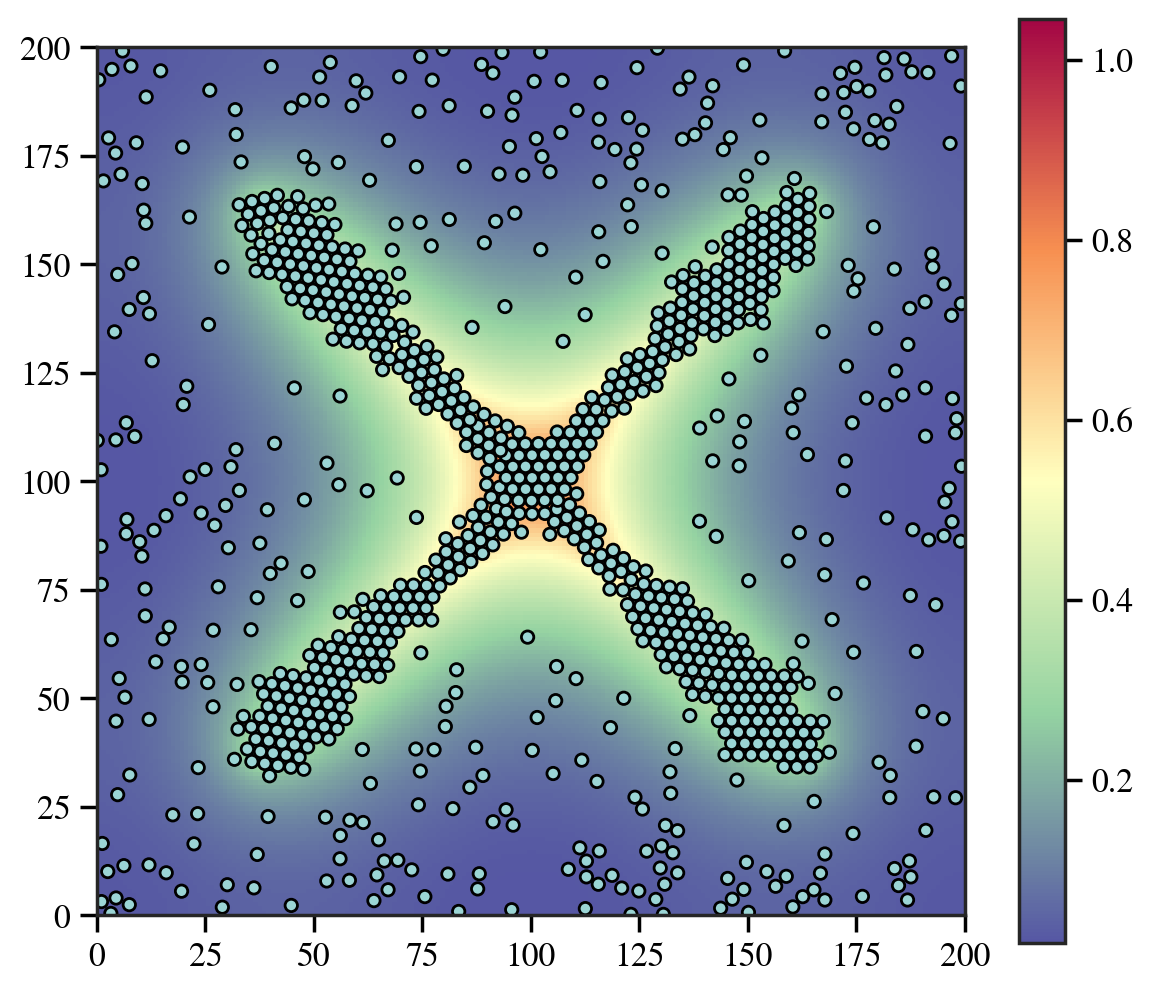
\includegraphics[width=\linewidth]{figs/simpleModeling1.png}
    }
    \hfill
    \subcaptionbox{$d_n=10$}[0.49\linewidth]{
      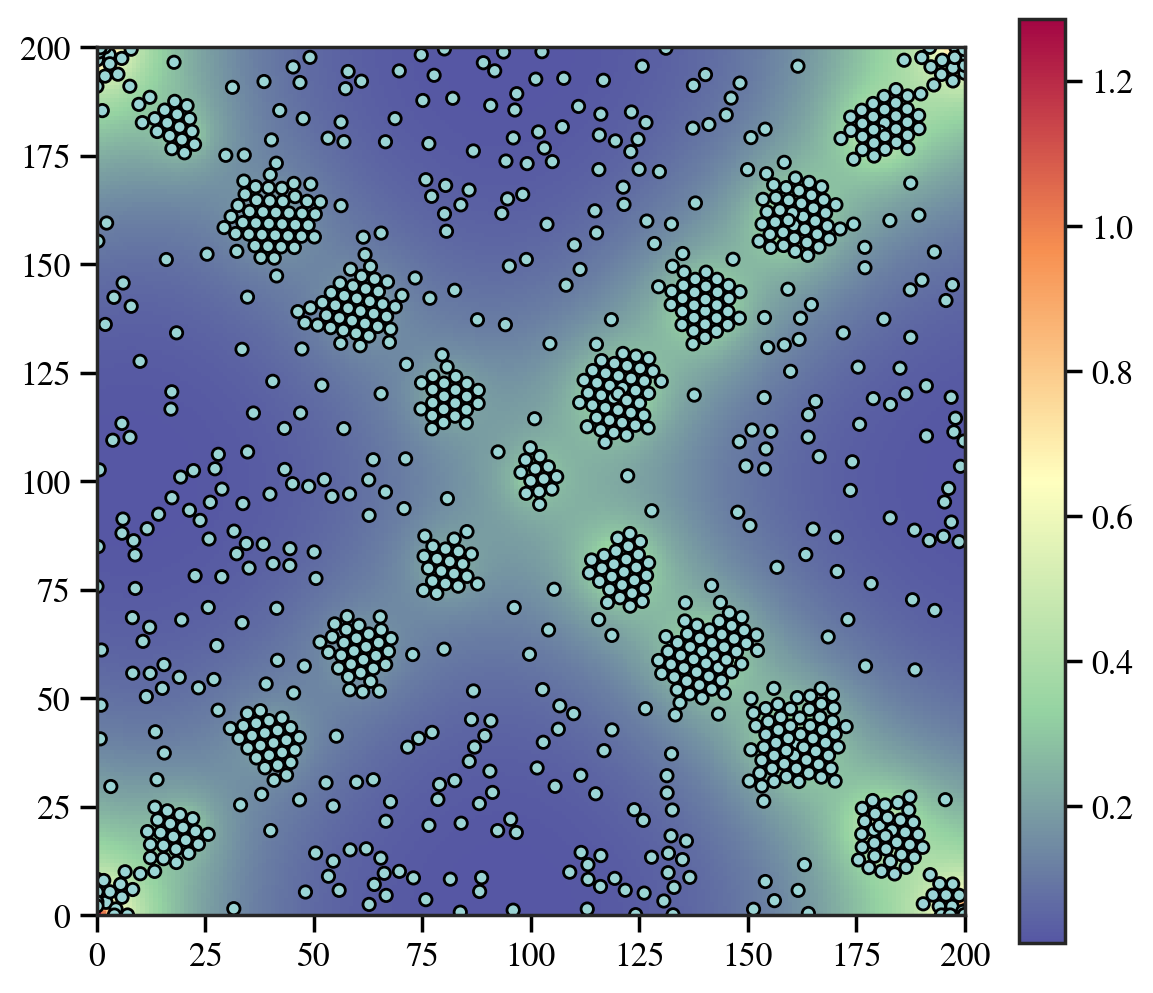
\includegraphics[width=\linewidth]{figs/simpleModeling2.png}
    }
    \caption{
        The simulation of the above model with $\alpha_c=-5$, $D_p=0$, $D_c=2$, $k_c=0.001$ and $\beta_c=0.3$. When the horizontal distance of nodes $d_n$ is small, the nodes are connected by the particles. While, when $d_n$ is large, the particles are not connected. 
    }
\end{figure}

Add new chemical $u$ to the model, which is produced by the particles and decays with time. The chemical $u$ will also affect the movement of the particles.
\begin{subequations}
    \begin{align}
        &\dot{\mathbf{r}}_i\left( t \right) =\alpha _u\nabla u+\alpha _c\nabla c-\nabla _{\mathbf{r}_i}V+\sqrt{2D_p}\mathbf{\eta }_i\\
        &\dot{u}\left( \mathbf{r},t \right) =D_u\nabla ^2c-k_uu+\beta _u\sum\nolimits_i^{}{\delta \left( \mathbf{r}-\mathbf{r}_i \right)}\\
        &\dot{c}\left( \mathbf{r},t \right) =D_c\nabla ^2c-k_cc+\beta _c\sum\nolimits_j^{}{\delta \left( \mathbf{r}-\mathbf{r}_{j}^{*} \right)}
    \end{align}
\end{subequations}

New ideas:
\begin{itemize}
    \item \textbf{Reverse density production}: too high density of particles will lead to the decrease of the production rate of the chemical.
    \item \textbf{Nonlinear coupling and decay}: the chemical $u$ will decay when $c$ is too high (\textcolor{red}{almost useless}).
    \begin{equation}
        \dot{u}\left( \mathbf{r},t \right) =D_u\nabla ^2c-\left( k_u+\gamma c \right) u+\beta _u\frac{c}{K_1+c}\cdot \frac{K_2}{K_2+c}\sum\nolimits_i^{}{\delta \left( \mathbf{r}-\mathbf{r}_i \right)}
    \end{equation}
\end{itemize}

\subsection{Definitions}
% \subsubsection{General Model}
\begin{subequations}
    \begin{align}
        &\dot{\mathbf{r}}_i\left( t \right) =\alpha _u\nabla u+\alpha_v \nabla v-\nabla _{\mathbf{r}_i}V+\sqrt{2D_p}\mathbf{\eta }_i\\
        &\dot{u}\left( \mathbf{r},t \right)=D_u\nabla ^2u-uv^2+k_f\left( 1-u \right) +k_u\sum\nolimits_i^{}{\delta \left( \mathbf{r}-\mathbf{r}_i \right)}+\beta _u\sum\nolimits_i^{}{\delta \left( \mathbf{r}-\mathbf{r}_{i}^{*} \right)}\\
        &\dot{v}\left( \mathbf{r},t \right)=D_v\nabla ^2v+uv^2-k_dv+k_v\sum\nolimits_i^{}{\delta \left( \mathbf{r}-\mathbf{r}_i \right)}+\beta _v\sum\nolimits_i^{}{\delta \left( \mathbf{r}-\mathbf{r}_{i}^{*} \right)}
    \end{align}
\end{subequations}
for $i=1,2,\cdots,N$. Here, $\mathbf{r}_i$ is the position of the $i$-th particle, $D_{u,v}$ is the diffusion coefficient, $k_{f,d}$ is the production rate, $k_{u,v}$ is the degradation rate, $\alpha _u$ and $\alpha$ are the chemotactic sensitivity, $V$ is the potential field, $\beta _{u,v}$ is the chemotactic sensitivity to the target, and $\mathbf{\eta }_i$ is a Gaussian white noise with zero mean and unit variance.
\begin{subequations}
    \begin{align}
        &\dot{\mathbf{r}}_i\left( t \right) =\alpha _u\nabla u+\alpha_v \nabla v+\alpha_c \nabla c-\nabla _{\mathbf{r}_i}V+\sqrt{2D_p}\mathbf{\eta }_i\\
        &\dot{u}\left( \mathbf{r},t \right) =D_u\nabla ^2u-uv^2+k_f\left( 1-u \right) +k_u\sum\nolimits_i^{}{\delta \left( \mathbf{r}-\mathbf{r}_i \right)}\\
        &\dot{v}\left( \mathbf{r},t \right) =D_v\nabla ^2v+uv^2-k_dv+k_v\sum\nolimits_i^{}{\delta \left( \mathbf{r}-\mathbf{r}_i \right)}\\
        &\dot{c}\left( \mathbf{r},t \right) =D_c\nabla ^2c-k_cc+\beta _c\sum\nolimits_i^{}{\delta \left( \mathbf{r}-\mathbf{r}_{i}^{*} \right)}
    \end{align}
\end{subequations}


\section{Continuum model}

\newpage
\section{Behaviors}

\bibliography{ref}

\end{document}